% ------- Flag di Debug  ---------------------------------------------------------------------------
\newif\ifToninus
\newcommand{\comment}[1]{\ifToninus\textcolor{gray}{\small{\textit{#1}}}\fi}
\Toninustrue

%- D0cum3nt ----------------------------------------------------------------------------------------------------------------------------------
\ifToninus
\documentclass[8pt,handout]{beamer}
\else
\documentclass[9pt]{beamer}
\fi

%- T1tle--------------------------------------------------------------------------------------------------------------------------
	\title{An invitation to Geometric Mechanics}
	\author{Antonio Michele Miti}
	\date{28 November 2017}

%- Packages ---------------------------------------------------------------------------------------------------------------------------
%			Standalone non funziona ancora bene con beamer.
\usepackage[mode=buildnew]{standalone}				%\includestandalone[width=\textwidth]{../Pictures/GeometricPicture0}
\usepackage{tikz}
\usepackage{pgfplots}
\pgfplotsset{compat=newest}
\usepackage{amsfonts}
\usepackage{xcolor}
\usepackage[utf8]{inputenc}
%\usepackage{fourier}							%\bomb \danger symbol
%\usepackage{arev}								%\smileface \sadface
\usepackage{animate}
\usepackage{appendixnumberbeamer}
\usepackage{mathtools}


%--Beamer Style--------------------------------------------------------------------------------------------------------------------------------
\usetheme{Copenhagen}

% FootLine
\setbeamertemplate{footline}[frame number]

%Headline
\setbeamertemplate{headline}{%
\leavevmode%
  \hbox{%
    \begin{beamercolorbox}[wd=\paperwidth,ht=2.5ex,dp=1.125ex]{palette quaternary}%
    \insertsectionnavigationhorizontal{\paperwidth}{}{\hskip0pt plus1filll}
    \end{beamercolorbox}%
  }
}

%Navigation Bar
\beamertemplatenavigationsymbolsempty



%Common symbols
\usepackage[diffgeo,geomec,aqft,ldpo,genrel,cat]{toninus-math-symbols}
%---------------------------------------------------------------------------------------------------------------------------------------------------------------------

%\usetheme{CambridgeUs}





\begin{document}


%\/\/\/\/\/\/\/\/\/\/\/\/\/\/\/\/\/\/\/\/\/\/\/\/\/\/\/\/\/\/\/\/\/\/\/\/\/\/\/\/\/\/\/\/\/\/\/\/\/\/\/\/\/\/\/\/\/\/\/\/\/\/\/\/\/\/\/\/\/
%				Intro
%\/\/\/\/\/\/\/\/\/\/\/\/\/\/\/\/\/\/\/\/\/\/\/\/\/\/\/\/\/\/\/\/\/\/\/\/\/\/\/\/\/\/\/\/\/\/\/\/\/\/\/\/\/\/\/\/\/\/\/\/\/\/\/\/\/\/\/\/\/
%\section*{Intro}	

\ifToninus
%	\frame{\titlepage}
\else
	\frame{\titlepage}
\fi

\ifToninus
	\begin{frame}{Overview}
		\tableofcontents
	\end{frame}
\else

\fi

\section{Intro}	

	\begin{frame}
		\frametitle{What is Geometric Mechanics?}
		\begin{block}<1->{As a branch of \emph{Applied Mathematics}}
			Employs modern (differential) geometry to the description of physical systems	.		
		\end{block}
		\begin{block}<2->{As an approach to \emph{Rational Mechanics}:}
			\begin{itemize}
				\item \textbf{Key idea:} make use of geometry in order to encode completely the mechanical property of a system regardless to the coordinate system employed.
				\item \textbf{The goal:} reconstruction of all physical observables of interest from these abstract mathematical setting.
				\item \textbf{Advantage:} formalize the relevant structure of the system in order to be able to reconstruct its quantum and relativistic counterpart.
			\end{itemize}
			
		\end{block}
			\begin{exampleblock}<3->{Some direct applications:}
			\begin{itemize}
				\item Theoretical chemistry \comment{ the geometric language permits to formalize the evolution of system composed of both quantum and classical degree of freedom (mesoscopic scale)}
				\item Control theory
				\item Image reconstruction
			\end{itemize}
			\end{exampleblock}


		%https://en.wikipedia.org/wiki/Geometric_mechanics

		%http://www10.mathematik.uni-wuerzburg.de/index.php?path=research/maphy

	\end{frame}

	\begin{frame}
		\frametitle{How does Geometry comes into Physics?}
		\begin{block}<2->{Trivial answer:}
			In describing our "physical space" in which all "physical systems" are embedded in.
		\end{block}
  	\begin{columns}<3->[T]
    	\begin{column}{.5\textwidth}
    		\begin{center}
					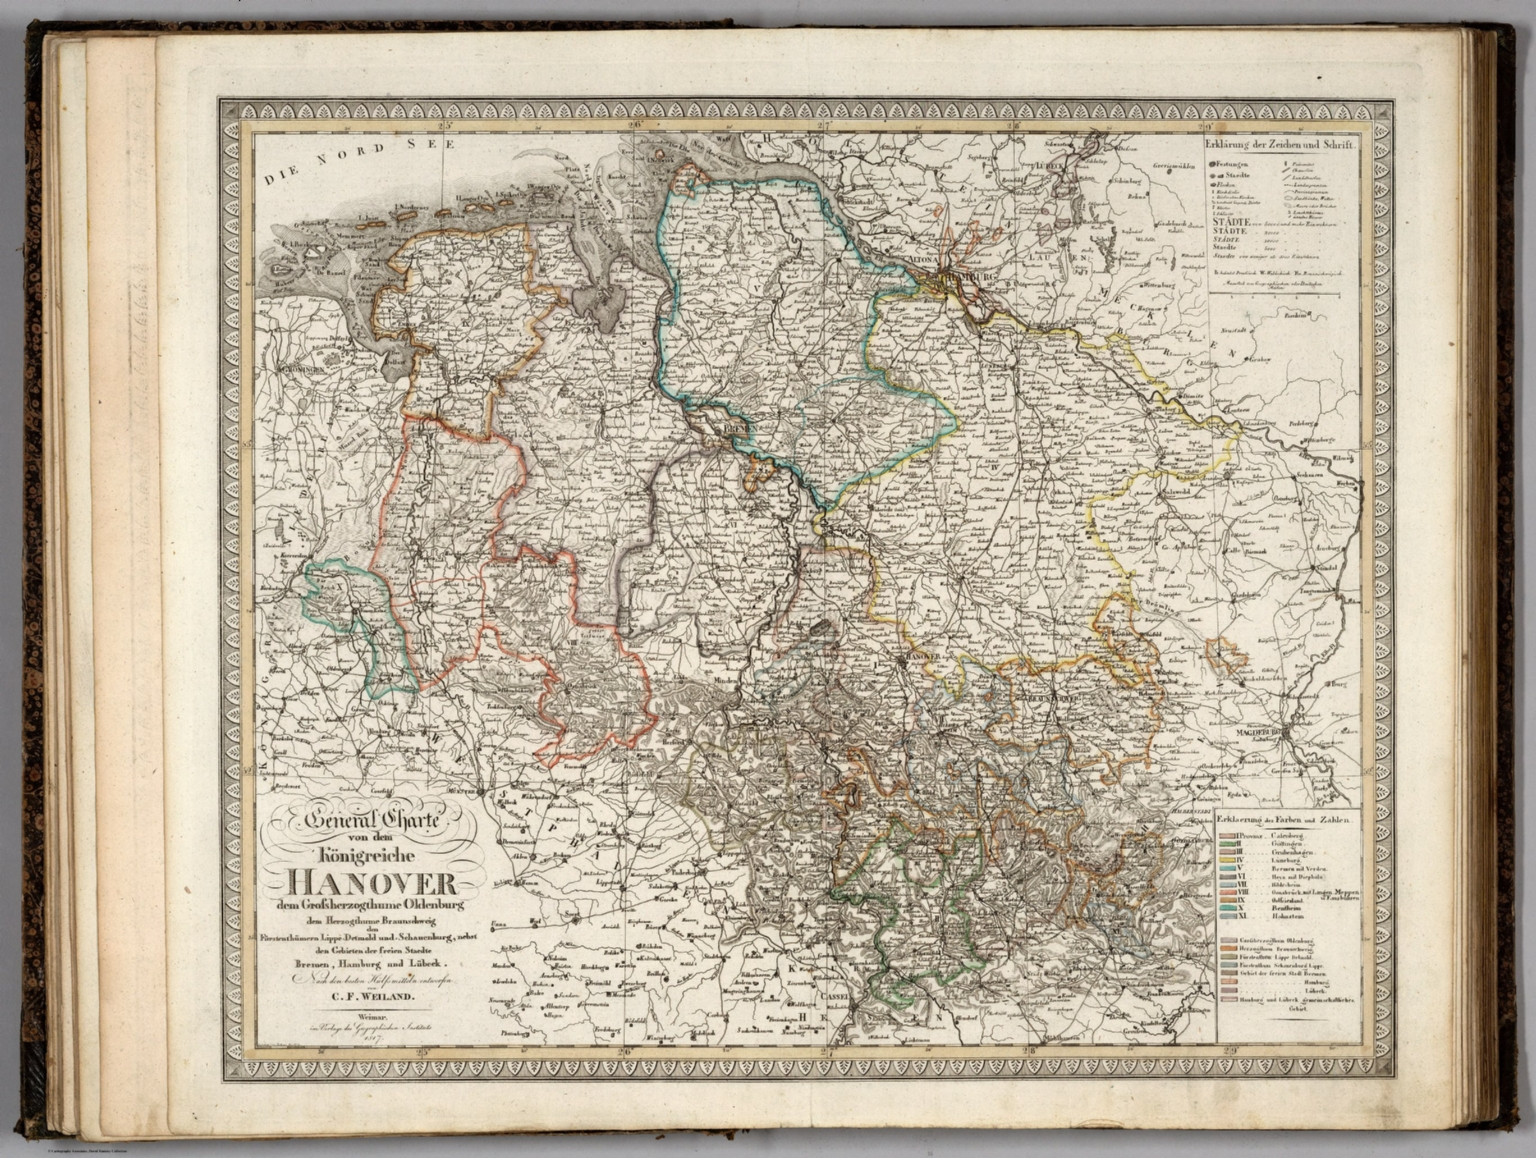
\includegraphics[width=0.9\textwidth]{Pics/map} 		
    		\end{center}
    	\end{column}
    	\begin{column}{.5\textwidth}
    			\vspace*{1em}
				\begin{exampleblock}{Historical fact:}
					Modern (intrinsic) differential geometry basically stemmed out from a Cartographic survey of the Kingdom of Hanover commissioned to Gauss.			
				\end{exampleblock}
				\comment{Nevertheless, the problem of measuring "Earth" is one of the oldest problem in mathematics}
    	\end{column}
    \end{columns}

		\comment{
		Nel 1818 fu chiesto a Gauss di compiere la rilevazione geodetica del Regno di Hannover, associandola ai precedenti rilevamenti effettuati in Danimarca.
La cartografia dell'Hannover portò Gauss a sviluppare la geometria differenziale insieme alle potenzialità della geometria non euclidea.
		}
				\begin{alertblock}<4->{There is much more!}
					Geometry provides a powerful language to encode deep properties of physics encompassing a huge variety of mechanical systems.
				\end{alertblock}
	
	\end{frame}

\section{Kinematics}
	\begin{frame}{Configuration Space}
  	\begin{columns}[T]
    	\begin{column}{.5\textwidth}		
				\includegraphics<1-2>[width=\textwidth]{Pics/GeoMec_Crop}
				\includegraphics<3->[width=\textwidth]{Pics/GeoMec_Crop_Noted}
    	\end{column}
    	\begin{column}{.5\textwidth}
				\comment{Consider the set of all possible admissible spatial displacements of a system}
				\begin{displaymath}				
    Q \coloneqq
    \left\{\parbox{45mm}{All possible admissible spatial displacements of a system.}
    \right\}.
				\end{displaymath}

 				\begin{block}<2->{Assumption 1:}
					For point particle $Q$ is a submanifold of $\Real^n$.
				\end{block}

 				\begin{block}<3->{Assumption 2:}
 Constraints are intrinsically encoded in the geometric structure of $Q$.
 				\end{block}
				
				\vfill
 				\begin{alertblock}<4->{Upshot:}
					$Q$ is a \emph{smooth manifold}. Configuration of a system are naturally described by points on it. Configuration coordinates are charts.
 				\end{alertblock}
			
    	\end{column}
  	\end{columns}	
	\end{frame}

	\begin{frame}{Trajectories}
  	\begin{columns}[T]
    	\begin{column}{.5\textwidth}		
				\begin{center}
					Double Pendulum:
  	  				\includegraphics<1->[width=\textwidth]{Pics/Fig4} 
    				\vspace{3em}
    				General system:
					\includegraphics<1->[width=\textwidth]{Pics/Fig2} 	
				\end{center}
    	\end{column}
    	\begin{column}{.5\textwidth}


 				\begin{alertblock}<2->{Upshot}
 					 Trajectories of the system can be described by smooth parametrized curves on $Q$
 					\begin{displaymath}
 						\Conf = C^\infty(\Real,Q)
 					\end{displaymath}
 				\end{alertblock}
 					\vspace{1em}
				\begin{center} 				
 					\includegraphics<2->[width=\textwidth]{Pics/KinematicalConfig}		
 				\end{center}
					
    	\end{column}
  	\end{columns}	
	\end{frame}

	\begin{frame}{Velocities}
  	\begin{columns}[T]
    	\begin{column}{.5\textwidth}		
				\begin{center}
					Double Pendulum:
  	  				\includegraphics<1->[width=\textwidth]{Pics/Fig5} 
    				\vspace{3em}
    				General system:
					\includegraphics<1->[width=\textwidth]{Pics/Fig3} 	
				\end{center}
    	\end{column}
    	\begin{column}{.5\textwidth}


 				\begin{alertblock}<2->{Upshot}
 					Instant velocities along a trajectory are \emph{tangent vectors} to the manifold $Q$
 					\begin{displaymath}
 						\dot{\gamma}(t) = V_{\gamma(t)} \in T_{\gamma(t)} Q
 					\end{displaymath}
 				\end{alertblock}
 				\begin{alertblock}<3->{Upshot}
					Collectively, all the possible tangent vector constitute another manifold called the \emph{Tangent Bundle}
					\begin{displaymath}
						TQ = \coprod_{q \in Q} T_q Q
					\end{displaymath}
 				\end{alertblock}
 					%\vspace{1em}
				\begin{center} 				
 					%\includegraphics<2->[width=\textwidth]{Pics/KinematicalConfig}		
 				\end{center}
    	\end{column}
  	\end{columns}	
	\end{frame}


\section{Dynamics}

	\begin{frame}{(Formal) Dynamics}
		\comment{We have all the ingredients to encode Dynamics in this geometrical settings.}
		\begin{exampleblock}<1->{Principle of least action}
			The path taken by the system between times $t_1$ and $t_2$ and configurations $q_1$ and $q_2$ is the one for which the action is stationary (no change) to first order.
		\end{exampleblock}
    		\begin{alertblock}<2->{Upshot}
    			All the interaction of the ambient on the system could be encoded in a \emph{action functional}:
    			$\qquad 				S: \Conf \rightarrow \Real  $
    		\end{alertblock}
  	\begin{columns}[T]
    	\begin{column}{.5\textwidth}		
				\begin{flushleft}
							\includegraphics<1>[width=1.1\textwidth]{Pics/CovDyn1} 
							\includegraphics<2>[width=1.1\textwidth]{Pics/CovDyn2} 	
							\includegraphics<3->[width=1.1\textwidth]{Pics/CovDyn3} 			
				\end{flushleft}						
		
    	\end{column}
    	\begin{column}{.5\textwidth}	
			\begin{alertblock}<3->{Upshot}
				Extremal conditions:
				\begin{displaymath}
					\frac{\delta}{\delta \gamma} S = 0
				\end{displaymath}
				\comment{$\Conf$ it is best understood as an infinite dimensional space, 
					differential calculus (a.k.a. variational calculus) on it \emph{should} be performed with care!}
				yields a differential operator
				\begin{displaymath}
					P: \Conf \rightarrow \Conf
				\end{displaymath}
				containing all the information about the dynamical evolution of the system.
				\comment{ (N.b. operator $P$ is not valued on $C$ but on k-holonomic section with k order of $P$.)}   	
			\end{alertblock}
    	\end{column}
  	\end{columns}	
		
	\end{frame}

	\begin{frame}{Lagrangian dynamics}
		\comment{Practically we do not consider such general action functional, but we restrict to functional of this type}
		\begin{block}{Working condition:}
			Action is a \emph{Lagrangian functional}:
			$ 	S [\gamma]= \int_\Real L(t,\gamma^i, \dot{\gamma}^i) dt $
		\end{block} 
		\comment{
			This is also motivated from stability condition of solutions (Ostragdsky)
		}

  	\begin{columns}[T]
    	\begin{column}{.5\textwidth}	
    	\begin{itemize}
    		\item     	The \emph{"Motion opertor"} results in:
				\begin{displaymath}
					P= \frac{d}{dt}\big(\frac{\partial}{\partial \dot{\gamma}^i}L\big)-\frac{\partial}{\partial \gamma^i}L \qquad \textrm{\tiny(Euler-Lagrange)}
				\end{displaymath}
			\item<2-> 	Equations could be integrated (giving a natural motion of the system),
						fixing a pair $(q,v)$ of configuration and (generalized) velocity.
    	\end{itemize}

		\begin{alertblock}<3->{Upshot}
			(Lagrangian) states are points in $TQ$.\\
			Lagrangian dynamics is encoded in a smooth function $L: TQ \rightarrow \Real$.
		\end{alertblock}
    	\end{column}
    	\begin{column}{.5\textwidth}
				\begin{center} 				
 					\includegraphics<3->[width=0.75\textwidth]{Pics/LagDyn}		\end{center}
    	\end{column}
  	\end{columns}			
		
	\end{frame}


	\begin{frame}{Hamiltonian dynamics}
  	\begin{columns}[T]
    	\begin{column}{.5\textwidth}	
    	Basic Idea: instead of fixing a state via its velocity we use \emph{conjugate momenta}.
			\comment{
				Instead of using $\dot{q}$ which determines the rat of change in the system configuration we employ a description in the change of the system's kinetic energy
				$L = T - V \quad\Rightarrow\quad \frac{\partial}{\partial \dot{q}}L = \frac{\partial}{\partial \dot{q}}T$
			}
		\begin{exampleblock}<2->{Momenta are \emph{co-vectors}.}
			\begin{itemize}
				\item Force is a linear form:
						$F : v_p \mapsto L $ "infinitesimal work"
				\item 
					A conservative force yields a potential:
					$d V = F = \dot{p} = \mathcal{L}_v p$
				\item $p$ is a 1-form.
			\end{itemize}
		\end{exampleblock}
		\comment{if you are not conviced of it recall how conjugate momenta is defines from a lagrangian and note that its componet are covariant}
		
		\begin{alertblock}<3->{Upshot}
			(Hamiltonian) states are point in $T^\ast Q$.\\
			Hamiltonian dynamics is encoded in a smooth function $H: T^\ast Q \rightarrow \Real$.
		\end{alertblock}
		\begin{itemize}
			\item<4-> $M = T^\ast Q$ is known as \emph{Phase Space}
		\end{itemize}


    	\end{column}
    	\begin{column}{.5\textwidth}
				\begin{center} 				
 					\includegraphics<3->[width=0.9\textwidth]{Pics/HamDyn}		\end{center}
    	\end{column}
  	\end{columns}				
	\end{frame}

\section{Symmetries}
	\begin{frame}{Symplectic Geometry}
		\begin{exampleblock}{Key point}
			$T^\ast Q$ it's naturally symplectic (i.e. endowed with a closed, bilinear, skew-symmetric form).\\
			\underline{Abstraction}: Mechanical systems $\quad \mapsto \quad$ symplectic manifold $(M,\omega)$.
		\end{exampleblock}

  	\begin{columns}[T]
    	\begin{column}{.5\textwidth}	
							\includegraphics<1>[width=1.1\textwidth]{Pics/Fig7} 
							\includegraphics<2->[width=1.1\textwidth]{Pics/Fig8} 		
    	\end{column}
    	\begin{column}{.5\textwidth}
			\begin{itemize}
				\item<1-> Classical observables are elements in $C^\infty(M,\Real)$
				\item<2-> Observable yields hamiltonian fields $\textrm{d} H = \omega(X_H, \cdot)$
				\item<3-> Trajectories are integral flows of $X_H$
			\end{itemize}

    	\end{column}
  	\end{columns}				
		
	
		
		
	\end{frame}

	\begin{frame}{Geometry of symmetries}
		\comment{Ok, basic mechanical structures are encoded in geometry. but there is another complementary geometrical property that's natural in physics: symmetry}
		\begin{alertblock}{Upshot}
			Continous symmetries are described by actions of a Lie group on $M$.
		\end{alertblock}
		\begin{block}<2->{Noether}
			Presence of symmetries $\quad \Rightarrow \quad$ existence of conserved quantities.
		\end{block}	
  	\begin{columns}[T]
    	\begin{column}{.5\textwidth}
    	\begin{block}<3->{Symplectic reduction}
       	System dynamics should be restricted to level set of conserved observables in order to efficiently store dynamical properties.\\
    	\end{block}
		\begin{block}<4->{Key concept:}
			Noether current are encoded in a \emph{moment map}  $\mu :M \rightarrow \mathfrak{g}^*$. This is the main tool for performing reduction.
			
		\end{block}
    	\end{column}
    	\begin{column}{.5\textwidth}	
    				\vspace{1em}
							\includegraphics<3->[width=1.1\textwidth]{Pics/Fig9} 
    	\end{column}
  	\end{columns}		
		
	\end{frame}



\section{Conclusions}
	\begin{frame}{Conclusions}
		\begin{alertblock}{Take away message}
			\begin{itemize}
				\item<1-> Manifolds arise naturally in the description of classical mechanical systems.
				\item<1-> Geometrization of mechanics yields an inherent intuition to differential geometry structures (manifolds, charts, vectors ...).
				\item<2-> Encoding a classical mechanical system via a precise mathematical framework allows  to the relevant structures of our physical theories to emerge.
				\item<2-> A sound mathematical foundation provides a solid ground where to perform axiomatization of physical theories, quantization and "relativization".
				\item<3-> With a slight refinement of the mathematical language, also systems with continuous degrees of freedom (fluid and fields) can be accommodated within this geometrical framework as well.
				\item<3-> This framework could be adapted directly to ordinary quantum mechanical systems (e.g. Bloch sphere).
			\end{itemize}
		\end{alertblock}
			
			\begin{itemize}
				\item[!!!]<4-> There are also  direct applications!!! (if you are that kind of person .... :P )
			\end{itemize}
			\comment{ If the priize of a complete mathematical foundation it's not enough for you...}

				
				
	\end{frame}

	\begin{frame}{Aknowledgments}

  	\begin{columns}[T]
    	\begin{column}{.5\textwidth}
		References;
		\begin{itemize}
			\item \href{http://arxiv.org/abs/1206.3302}{\emph{A Primer on Geometric Mechanics} -  C. Lessig - arXiv:1206.3302 }
		\end{itemize}
		Further Readings:
		\begin{itemize}
			\item Foundation of Mechanics - R. Abrham, J.E. Marsden.
			\item Introduction to Mechanics and Symmetries - J.E. Marsden, T. Ratiu
			\item Geometric Mechanics - R. Talman
			\item Geometry of Physics - T. Frankel
			\item Geometric Methods in Quantum Mechanics - M. Spera

		\end{itemize}
    	\end{column}
    	\begin{column}{.5\textwidth}	
    				\vspace{4em}
    				\begin{flushright}
							\includegraphics<2->[width=0.8\textwidth]{Pics/thankyou}   				
    				\end{flushright}
    	\end{column}
  	\end{columns}		



	\end{frame}

	\begin{frame}{Extended Bibliography}
			\nocite{*}
			\bibliography{biblio}
	\end{frame}

		
		

	\appendix
	\section{Extra}
	\frame{\sectionpage}

	\begin{frame}	% \danger : manca immagine
		\frametitle{Ordinary Canonical Formalism (Discrete degrees of freedom)}
  			\begin{columns}[T]
    			\begin{column}{.5\textwidth}
						\begin{enumerate}
							\item\emph{Configuration coordinates} $q^j$.
							\item\emph{Canonical conjugate momentai}  $p^j$.
							\item \emph{Symplectic matrix} \comment{(combinando $p^i,q^j$ in un'unica variabile $Q^I=\{q_1,\ldots, q_N ;p^1, \ldots, p^N\}$)}
								\begin{displaymath}
									\Omega=\begin{bmatrix}
										\begin{matrix}0 & 1\\ -1 & 0\end{matrix} & & 0 \\
											 & \ddots & \\
											 0 & & \begin{matrix}0 & 1 \\ -1 & 0
										\end{matrix}
									\end{bmatrix}
								\end{displaymath}
							\item \emph{Poisson brackets}: \comment{per 2 funzioni $A(Q^I) , B(Q^J)$}
								\begin{displaymath}
									\left\{A , B \right\} = \Omega^{I J} \frac{\partial A}{\partial Q^I} \frac{\partial B}{\partial Q^J}					
								\end{displaymath}
							\item \emph{Dynamics equations}
								\begin{displaymath}
									\left\{Q^I, H \right\} = \dot{Q}^I
								\end{displaymath}
							
								\comment{$$H(q,p) =  q \dot{q}(q,p)-L\left(q, \dot{q}(q,p)\right)$$}
								
								
						\end{enumerate}
    			\end{column}
    		   	\begin{column}{.5\textwidth}
					\parbox[c][.7\textheight][c]{\columnwidth}{%
						\comment{Animazione Pendolo con orbita rappresentata nel piano simplettico}
						\animategraphics[autoplay,loop,width=\textwidth]{3}{./Pics/SimpleHarmonicMotion/o_2830a51e4d07c739-}{0}{19}
 						\center \footnote{Ref: 
 							\href{https://en.wikibooks.org/wiki/A-level_Physics_(Advancing_Physics)/Simple_Harmonic_Motion}{en.wikibooks.org}}
  					}	
    			\end{column}
  			\end{columns}	
		\end{frame}

	\begin{frame}	% \danger : manca overlay: popup graduale degli elementi
		\frametitle{Canonical Intrinsic Formalism}
  			\begin{columns}[T]
    			\begin{column}{.5\textwidth}
    				\comment{Il formalismo a cui siamo abituati può essere visto in modo intrinsecamente generale globale usando gli strumenti  della geometria differenziale, varietà e spazi tangenti}
    					\begin{block}{Non-Covariant}
							\begin{itemize}
								\item Configurations space: $Q$. \comment{(le coordinate di configurazione sono un sistema di coordinate (non dire "carte locali".)}
								\item Spaze of generalized velocites: $TQ$. \comment{incollando tutti gli spazi tangenti}
								\item Phase space $T^*Q$. \comment{l'analogo per gli spazi duali, $Q^I$ sono una trivializzazione locale naturale)}
								\item $T^*Q$ it's naturally symplectic $\omega = dp^i \wedge dq^i$.
								\item Dynamics encoded in $L$ or $H$.\comment{Su TM è ambientata la dinamica lagrangiana e su T*M hamiltoniana.\\ sotto opportune condizioni sono equivalenti, }
							\end{itemize}
						\end{block}
						\begin{block}<2->{Covariant}
    					\comment{ Facciamo un Cambio di prospettiva: non più conformazioni "statiche" ma considero tutti i moti possibili}
							\begin{itemize}
								\item Space of kinematics configurations: $\Conf$. \comment{è l'insieme di tutte i moti compatibili con la cinematica}
								\item Dynamics encoded in an action: $S:\Conf \rightarrow \Real$. \comment{l'azione la rivediamo come una mappa definita sui moti}
								\item Differential equations of motion: $ P$. \comment{ dal principio di minima azione discende un'equazione differenziale su $\Conf$}
								\item Space of dynamics configurations: $\Sol$. \comment{Insieme delle equazioni del moto}		
							\end{itemize}
						\comment{\\accenno: quello che si sta facendo ricorda in un certo senso il passaggio dalla pittura di schrodinger a quella di heisnberg}
						\comment{\\difficoltà: queste varietà sono infinito dimensionali}	
						\end{block}
    			\end{column}
    		   	\begin{column}{.5\textwidth}
    		   		\vspace{1em}
    		   		\parbox[c][.7\textheight][c]{\columnwidth}{%
						\includegraphics<1>[width=\textwidth]{Pics/GeoMecFrameA}
						\includegraphics<2->[width=\textwidth]{Pics/GeoMecFrameB} 
					}
    			\end{column}
  			\end{columns}	
		\end{frame}
		

		\begin{frame}	% \danger : manca overlay: popup graduale degli elementi
			\frametitle{Covariant formalism extended to fields}
  			\begin{columns}[T]
    			\begin{column}{.5\textwidth}
    				\comment{Il formalismo covariante intrinseco si estende facilmente a sistemi più generali!\\}
    				Idea for point particles:
    					\begin{itemize}
    						\item Space of all configurations:
    						    \begin{displaymath}
    								\underset{(\textrm{Manifold})}{Q} \quad \mapsto \quad 
    								\underset{(\textrm{Bundle})}{\Real \times Q}
    							\end{displaymath}
    						\comment{La cinematica non viene più fondata su  $Q$ ma su $\Real \times Q$ (fibrato di configurazione) 	triviale nel caso dei sistemi ordinari}
    						\item Kinematics configurations:
    							\begin{displaymath}
    								\underset{(\textrm{curves})}{\gamma: \Real \rightarrow Q} \quad \mapsto \quad 
    								\underset{(\textrm{sections})}{\gamma: \Real \rightarrow \Real\times Q}
    							\end{displaymath}
    					\end{itemize}	

    				\begin{block}<2->{Classical field theories}
 						\begin{itemize}
 							\item Base manifold is a \emph{spacetime} $M$.
 							\comment{La varietà base non è più $\Real$ ma un generico spaziotempo}
							\item Kinematics configuration are \emph{sections} $\gamma: M \rightarrow M \times F$.
								\comment{$F$ è lo spazio target dei possibili valori che può assumere il campo}
							\item Motion equations $P$ are extracted from a \emph{Lagrangian Density} $\Lagrangian$ \comment{ingloba la struttura dinamica}
							\item Dynamics configurations are solutions of $P$
						\end{itemize}   				
    				\end{block}
    			\end{column}
    		 
    		   	\begin{column}{.5\textwidth}
					\comment{Evidenziare uno alla volta gli oggetti che introduco}
						\includegraphics<1-> [width=\textwidth]{Pics/FieMecFrame} \\
						\includegraphics<2-> [width=\textwidth]{Pics/AbstractFieldTheory(pezzotta)} 
    			\end{column}
  			\end{columns}		
		\end{frame}

		\begin{frame}{A glimpse to geometric quantum Mechanics}
						\includegraphics<1-> [width=\textwidth]{Pics/Bloch} 
						\footnote{\href{http://www.soi.wide.ad.jp/class/20050012/slides/03/6.html}{}}			
		\end{frame}

	
\end{document}











